\section*{2. Theory}

\subsection*{Half Adder and Full Adder}
A \textbf{half adder} adds two bits $x$ and $y$ and produces a sum $S$ and a carry $C$. A \textbf{full adder} adds two significant bits $x$, $y$ and the carry $z$ from the previous lower significant bit:
\[
    \text{Half adder: } S = x \oplus y,\ \ C = x y; \qquad
    \text{Full adder: } S = x \oplus y \oplus z,\ \ C = x y + z (x \oplus y).
\]

\begin{table}[H]
\centering
\small
\begin{minipage}[t]{0.35\textwidth}
    \centering
    \begin{tabular}{c c | c c}
    \toprule
    $x$ & $y$ & $C$ & $S$ \\
    \midrule
    0 & 0 & 0 & 0 \\
    0 & 1 & 0 & 1 \\
    1 & 0 & 0 & 1 \\
    1 & 1 & 1 & 0 \\
    \bottomrule
    \end{tabular}
    \captionof{table}{Half adder}
\end{minipage}
\begin{minipage}[t]{0.35\textwidth}
    \centering
    \begin{tabular}{c c c | c c}
    \toprule
    $x$ & $y$ & $z$ & $C$ & $S$ \\
    \midrule
    0 & 0 & 0 & 0 & 0 \\
    0 & 0 & 1 & 0 & 1 \\
    0 & 1 & 0 & 0 & 1 \\
    0 & 1 & 1 & 1 & 0 \\
    1 & 0 & 0 & 0 & 1 \\
    1 & 0 & 1 & 1 & 0 \\
    1 & 1 & 0 & 1 & 0 \\
    1 & 1 & 1 & 1 & 1 \\
    \bottomrule
    \end{tabular}
    \captionof{table}{Full adder}
\end{minipage}
\end{table}

\subsection*{4-bit Binary Adder}
A binary adder produces the arithmetic sum of two binary numbers. An $n$-bit \textbf{ripple carry adder} is built from $n$ full adders connected in cascade: the output carry of each full adder is connected to the input carry of the next one.
\begin{figure}[H]
    \centering
    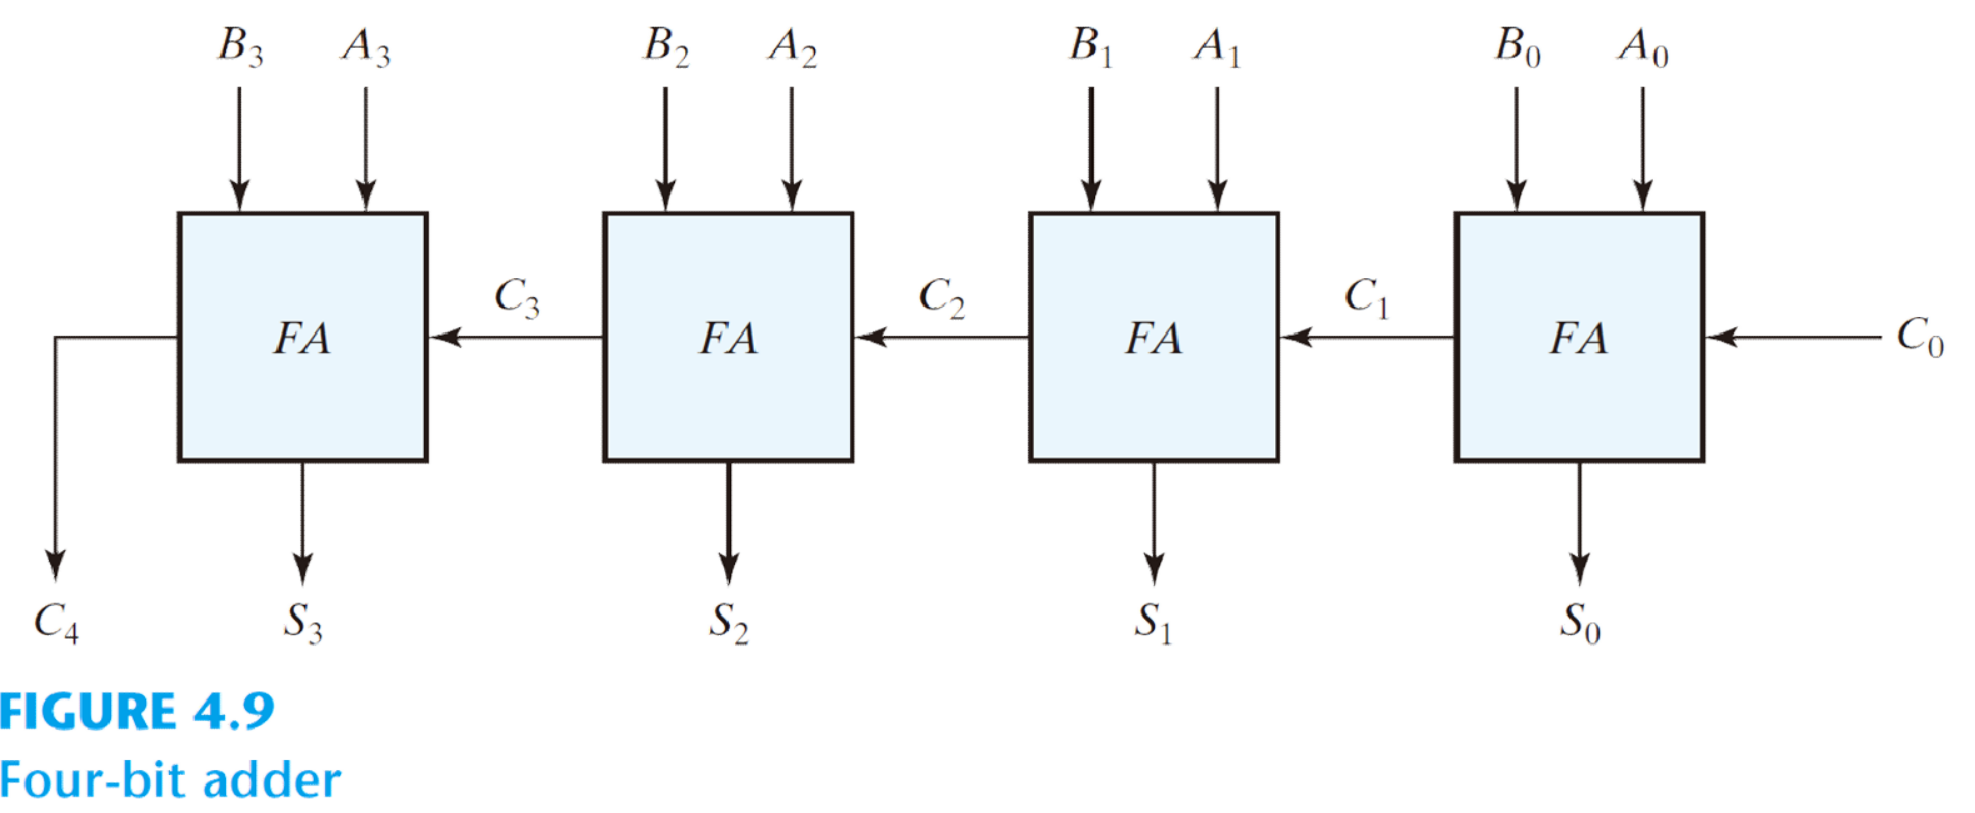
\includegraphics[width=0.7\textwidth]{pic/4bit_adder.png}
    \captionof{figure}{Four-bit ripple carry adder}
    \label{fig:4bit_adder}
\end{figure}

\subsection*{CD4008 4-bit Full Adder}
The CD4008 adds two 4-bit numbers $A_4A_3A_2A_1$ and $B_4B_3B_2B_1$ with a carry-in $C_1$, and outputs the sum $S_4S_3S_2S_1$ and the carry-out $C_O$. Instead of letting the carry ripple through all four stages, it uses a \textit{high-speed parallel carry} circuit to generate $C_O$. $V_{DD}$ (pin 16) is $+6\text{V}$ and $V_{SS}$ (pin 8) is ground.
\begin{figure}[H]
    \centering
    \begin{minipage}[c]{0.22\textwidth}
        \centering
        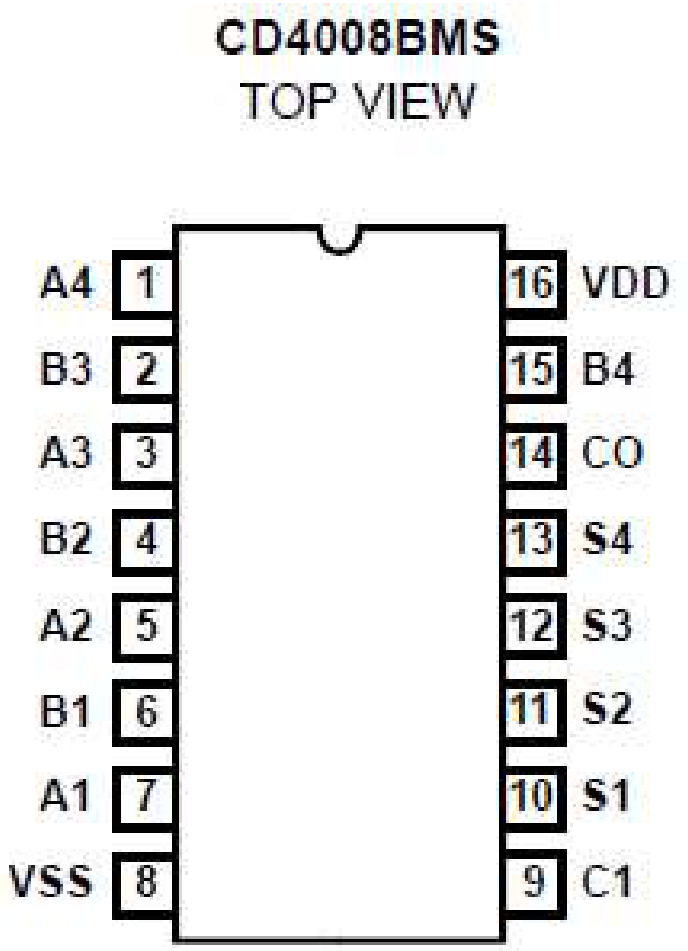
\includegraphics[width=\linewidth]{pic/cd4008_pin.png}
    \end{minipage}
    \hfill
    \begin{minipage}[c]{0.75\textwidth}
        \centering
        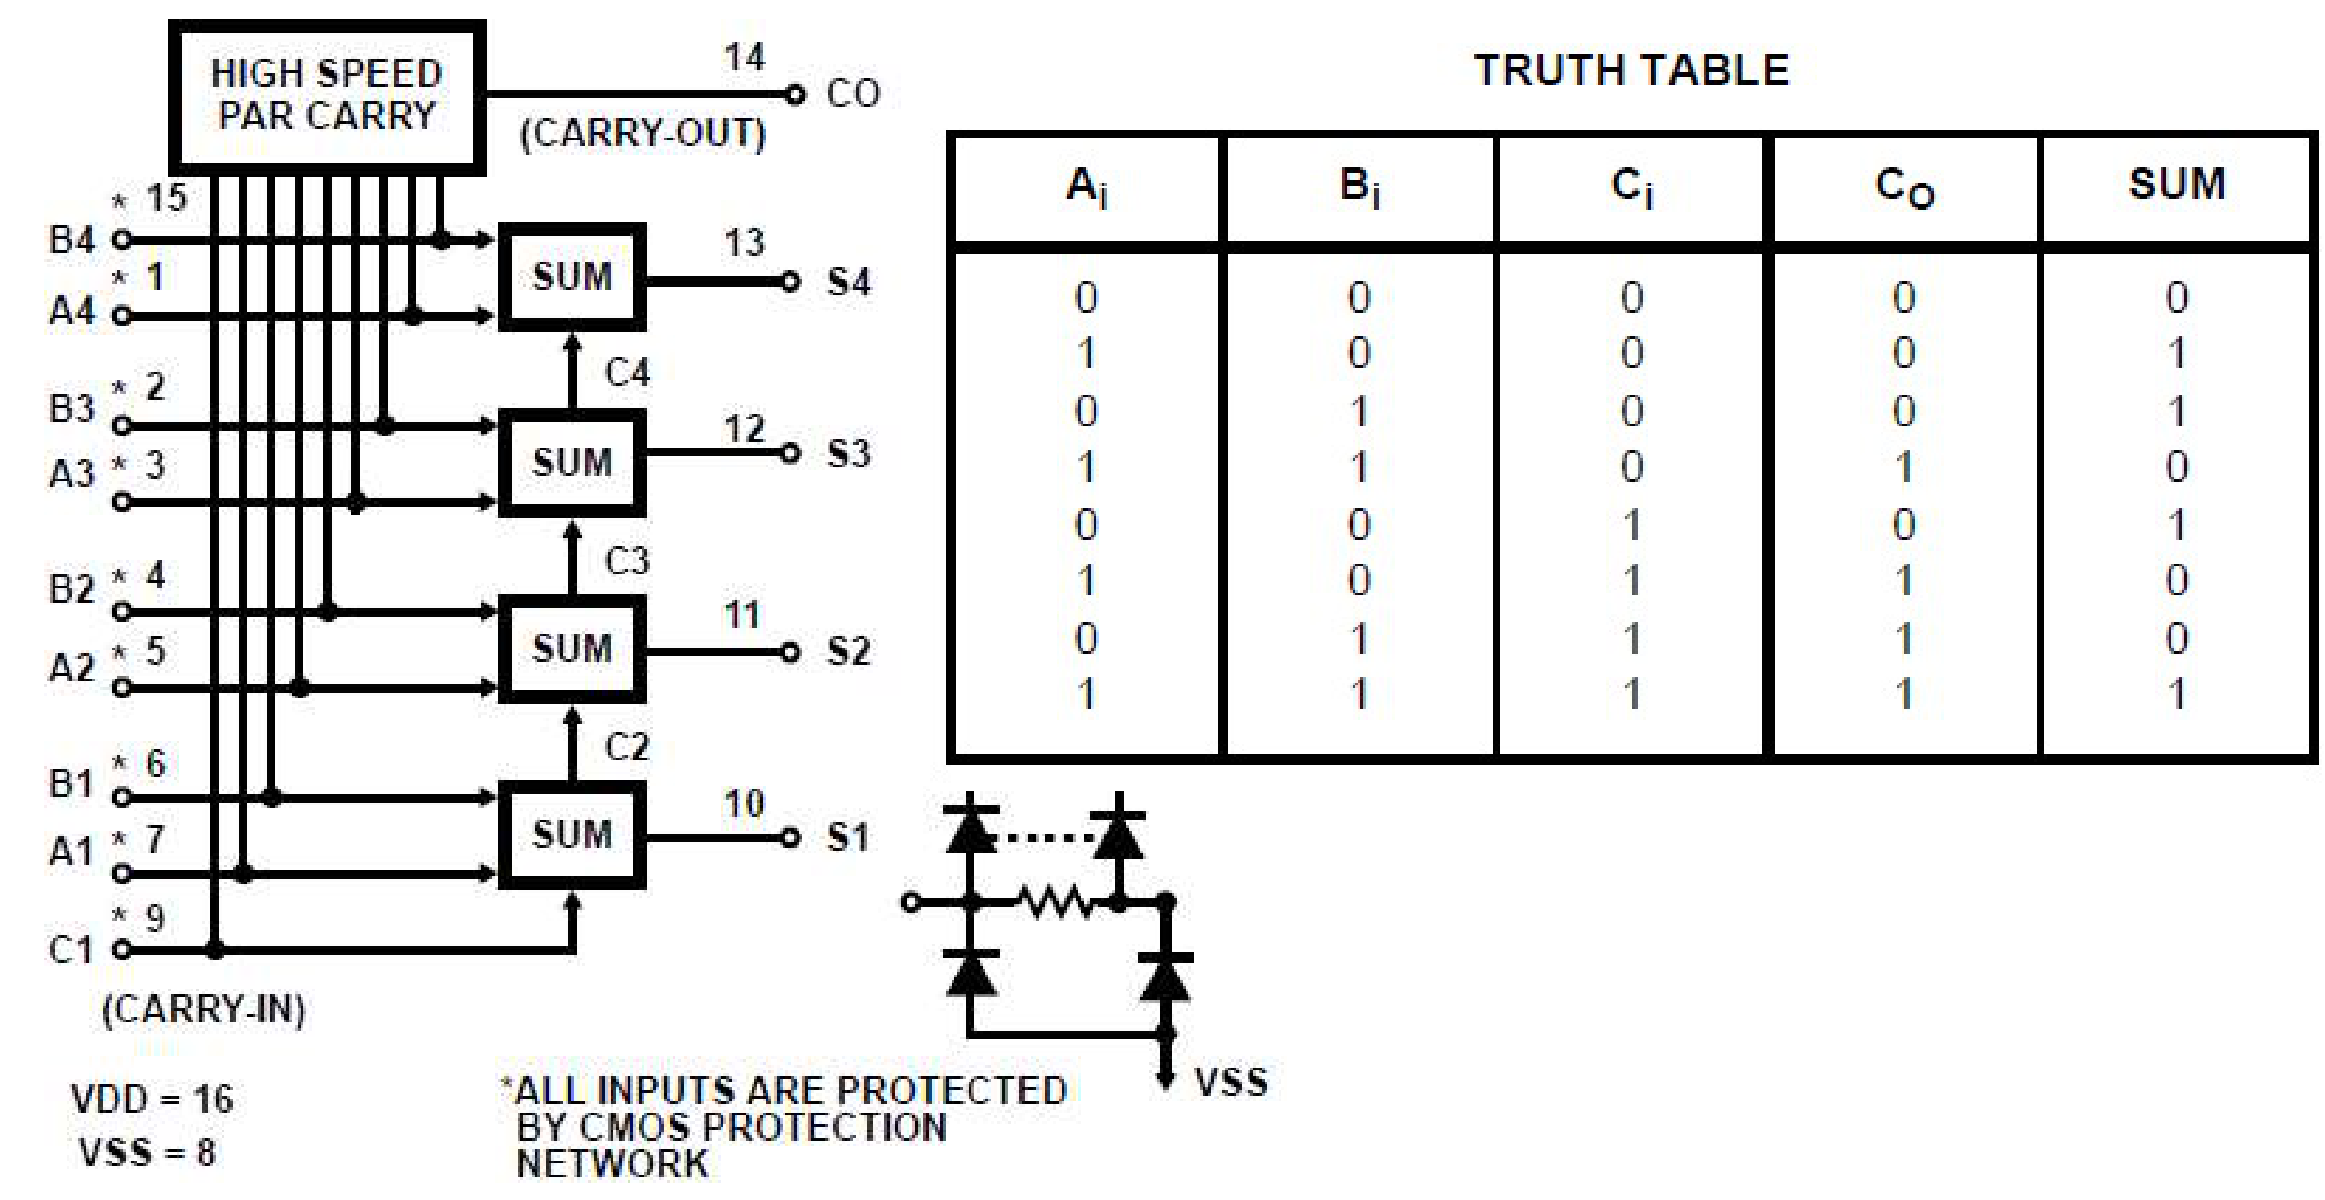
\includegraphics[width=\linewidth]{pic/cd4008_logic.png}
    \end{minipage}
    \captionof{figure}{CD4008 pin assignment (left), logic diagram and truth table (right)}
    \label{fig:cd4008}
\end{figure}

\subsection*{BCD and the CD4511 BCD-to-7-Segment Decoder}
Binary-coded decimal (BCD) represents each decimal digit 0--9 with a 4-bit code $0000 \sim 1001$. The CD4511 converts a BCD input $DCBA$ ($D$ is the MSB) into the seven segment signals $a \sim g$ (active high). For normal operation the control pins are set to lamp test $\overline{LT} = 1$, blanking $\overline{BI} = 1$ and latch enable $LE = 0$. Inputs $1010 \sim 1111$ are invalid BCD codes, and all segments are turned off. $V_{DD}$ (pin 16) is $+6\text{V}$; a larger $V_{DD}$ results in too large a current and may burn the device.

\begin{figure}[H]
    \centering
    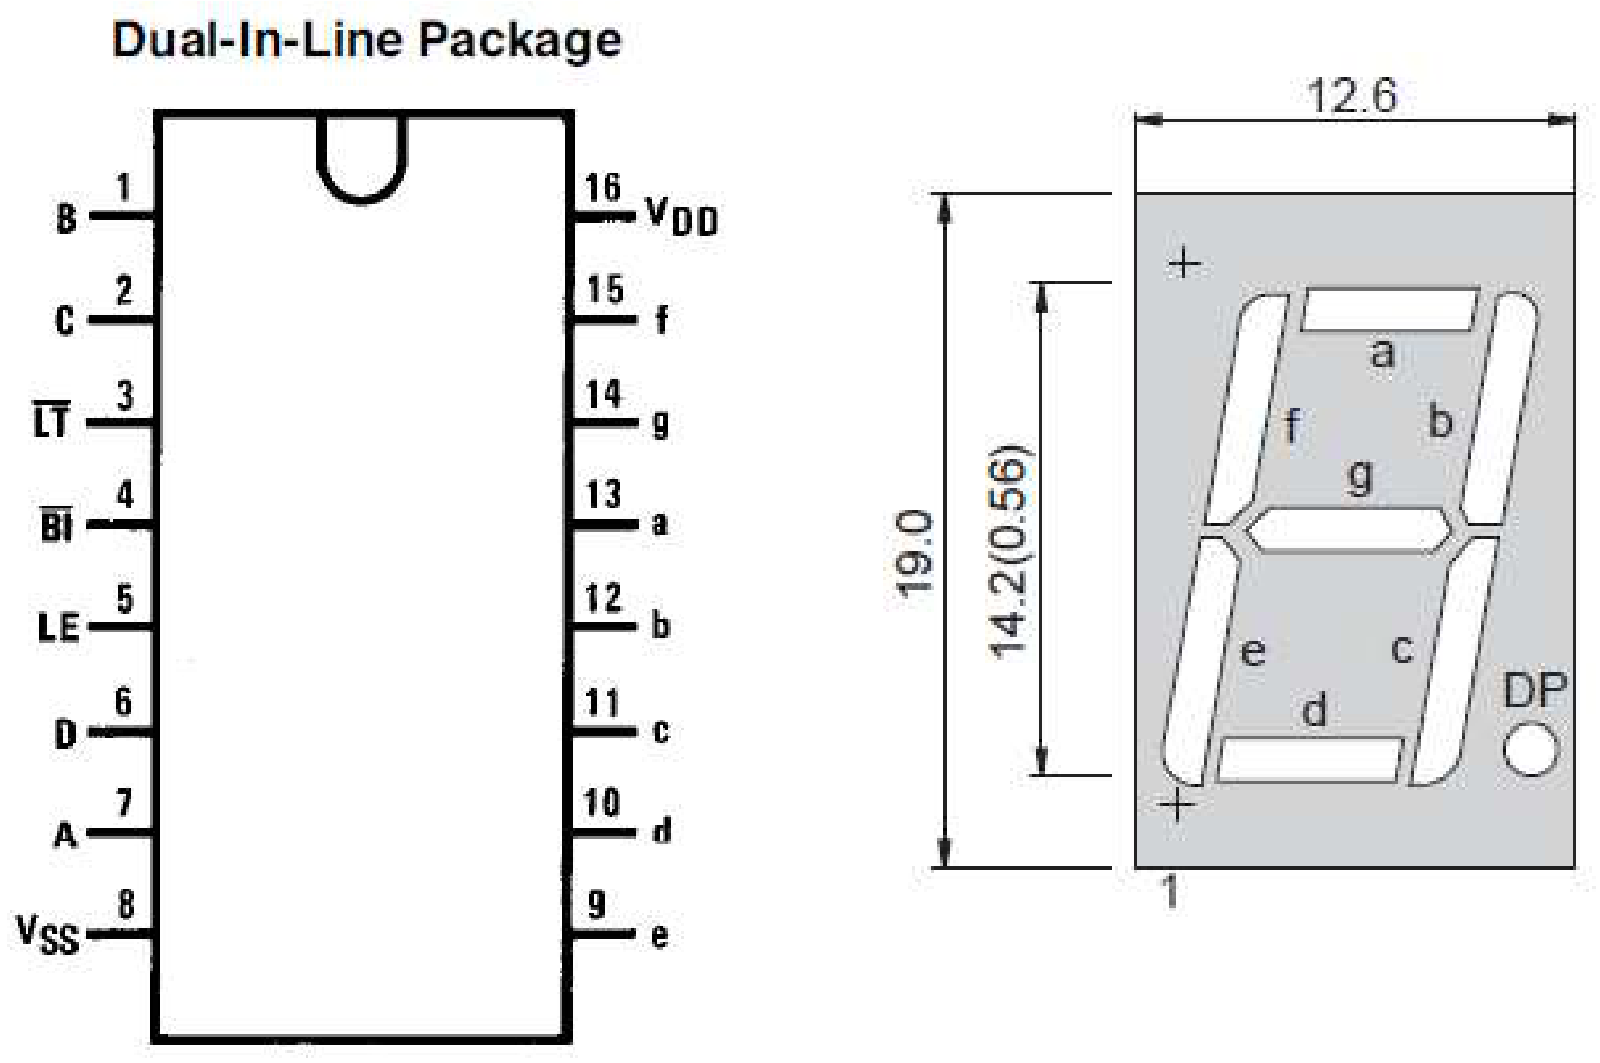
\includegraphics[width=0.6\textwidth]{pic/cd4511_pin.png}
    \captionof{figure}{CD4511 pin assignment (left) and 7-segment display (right)}
    \label{fig:cd4511}
\end{figure}

\begin{table}[H]
\centering
\small
\begin{tabular}{c c c c | c c c c c c c | c}
\toprule
$D$ & $C$ & $B$ & $A$ & $a$ & $b$ & $c$ & $d$ & $e$ & $f$ & $g$ & \textbf{Display} \\
\midrule
0 & 0 & 0 & 0 & 1 & 1 & 1 & 1 & 1 & 1 & 0 & 0 \\
0 & 0 & 0 & 1 & 0 & 1 & 1 & 0 & 0 & 0 & 0 & 1 \\
0 & 0 & 1 & 0 & 1 & 1 & 0 & 1 & 1 & 0 & 1 & 2 \\
0 & 0 & 1 & 1 & 1 & 1 & 1 & 1 & 0 & 0 & 1 & 3 \\
0 & 1 & 0 & 0 & 0 & 1 & 1 & 0 & 0 & 1 & 1 & 4 \\
0 & 1 & 0 & 1 & 1 & 0 & 1 & 1 & 0 & 1 & 1 & 5 \\
0 & 1 & 1 & 0 & 0 & 0 & 1 & 1 & 1 & 1 & 1 & 6 \\
0 & 1 & 1 & 1 & 1 & 1 & 1 & 0 & 0 & 0 & 0 & 7 \\
1 & 0 & 0 & 0 & 1 & 1 & 1 & 1 & 1 & 1 & 1 & 8 \\
1 & 0 & 0 & 1 & 1 & 1 & 1 & 0 & 0 & 1 & 1 & 9 \\
\bottomrule
\end{tabular}
\captionof{table}{CD4511 truth table for BCD 0--9 ($LE = 0$, $\overline{BI} = \overline{LT} = 1$)}
\label{tab:cd4511}
\end{table}

\subsection*{7-Segment Display}
A 7-segment display consists of seven LEDs ($a \sim g$) and a decimal point (DP). An LED is a pn-junction diode that emits light when it is forward biased. In a \textbf{common-cathode} display (used in this lab), all cathodes are connected to the common pins 3 and 8, which go to ground, and a segment lights when its anode is driven high. In a common-anode display the anodes are common and a segment lights when it is driven low. A $330\,\Omega$ resistor is connected in series with each segment to limit the LED current ($I = V/R$), so 7 resistors are needed.

\begin{figure}[H]
    \centering
    \begin{minipage}[c]{0.62\textwidth}
        \centering
        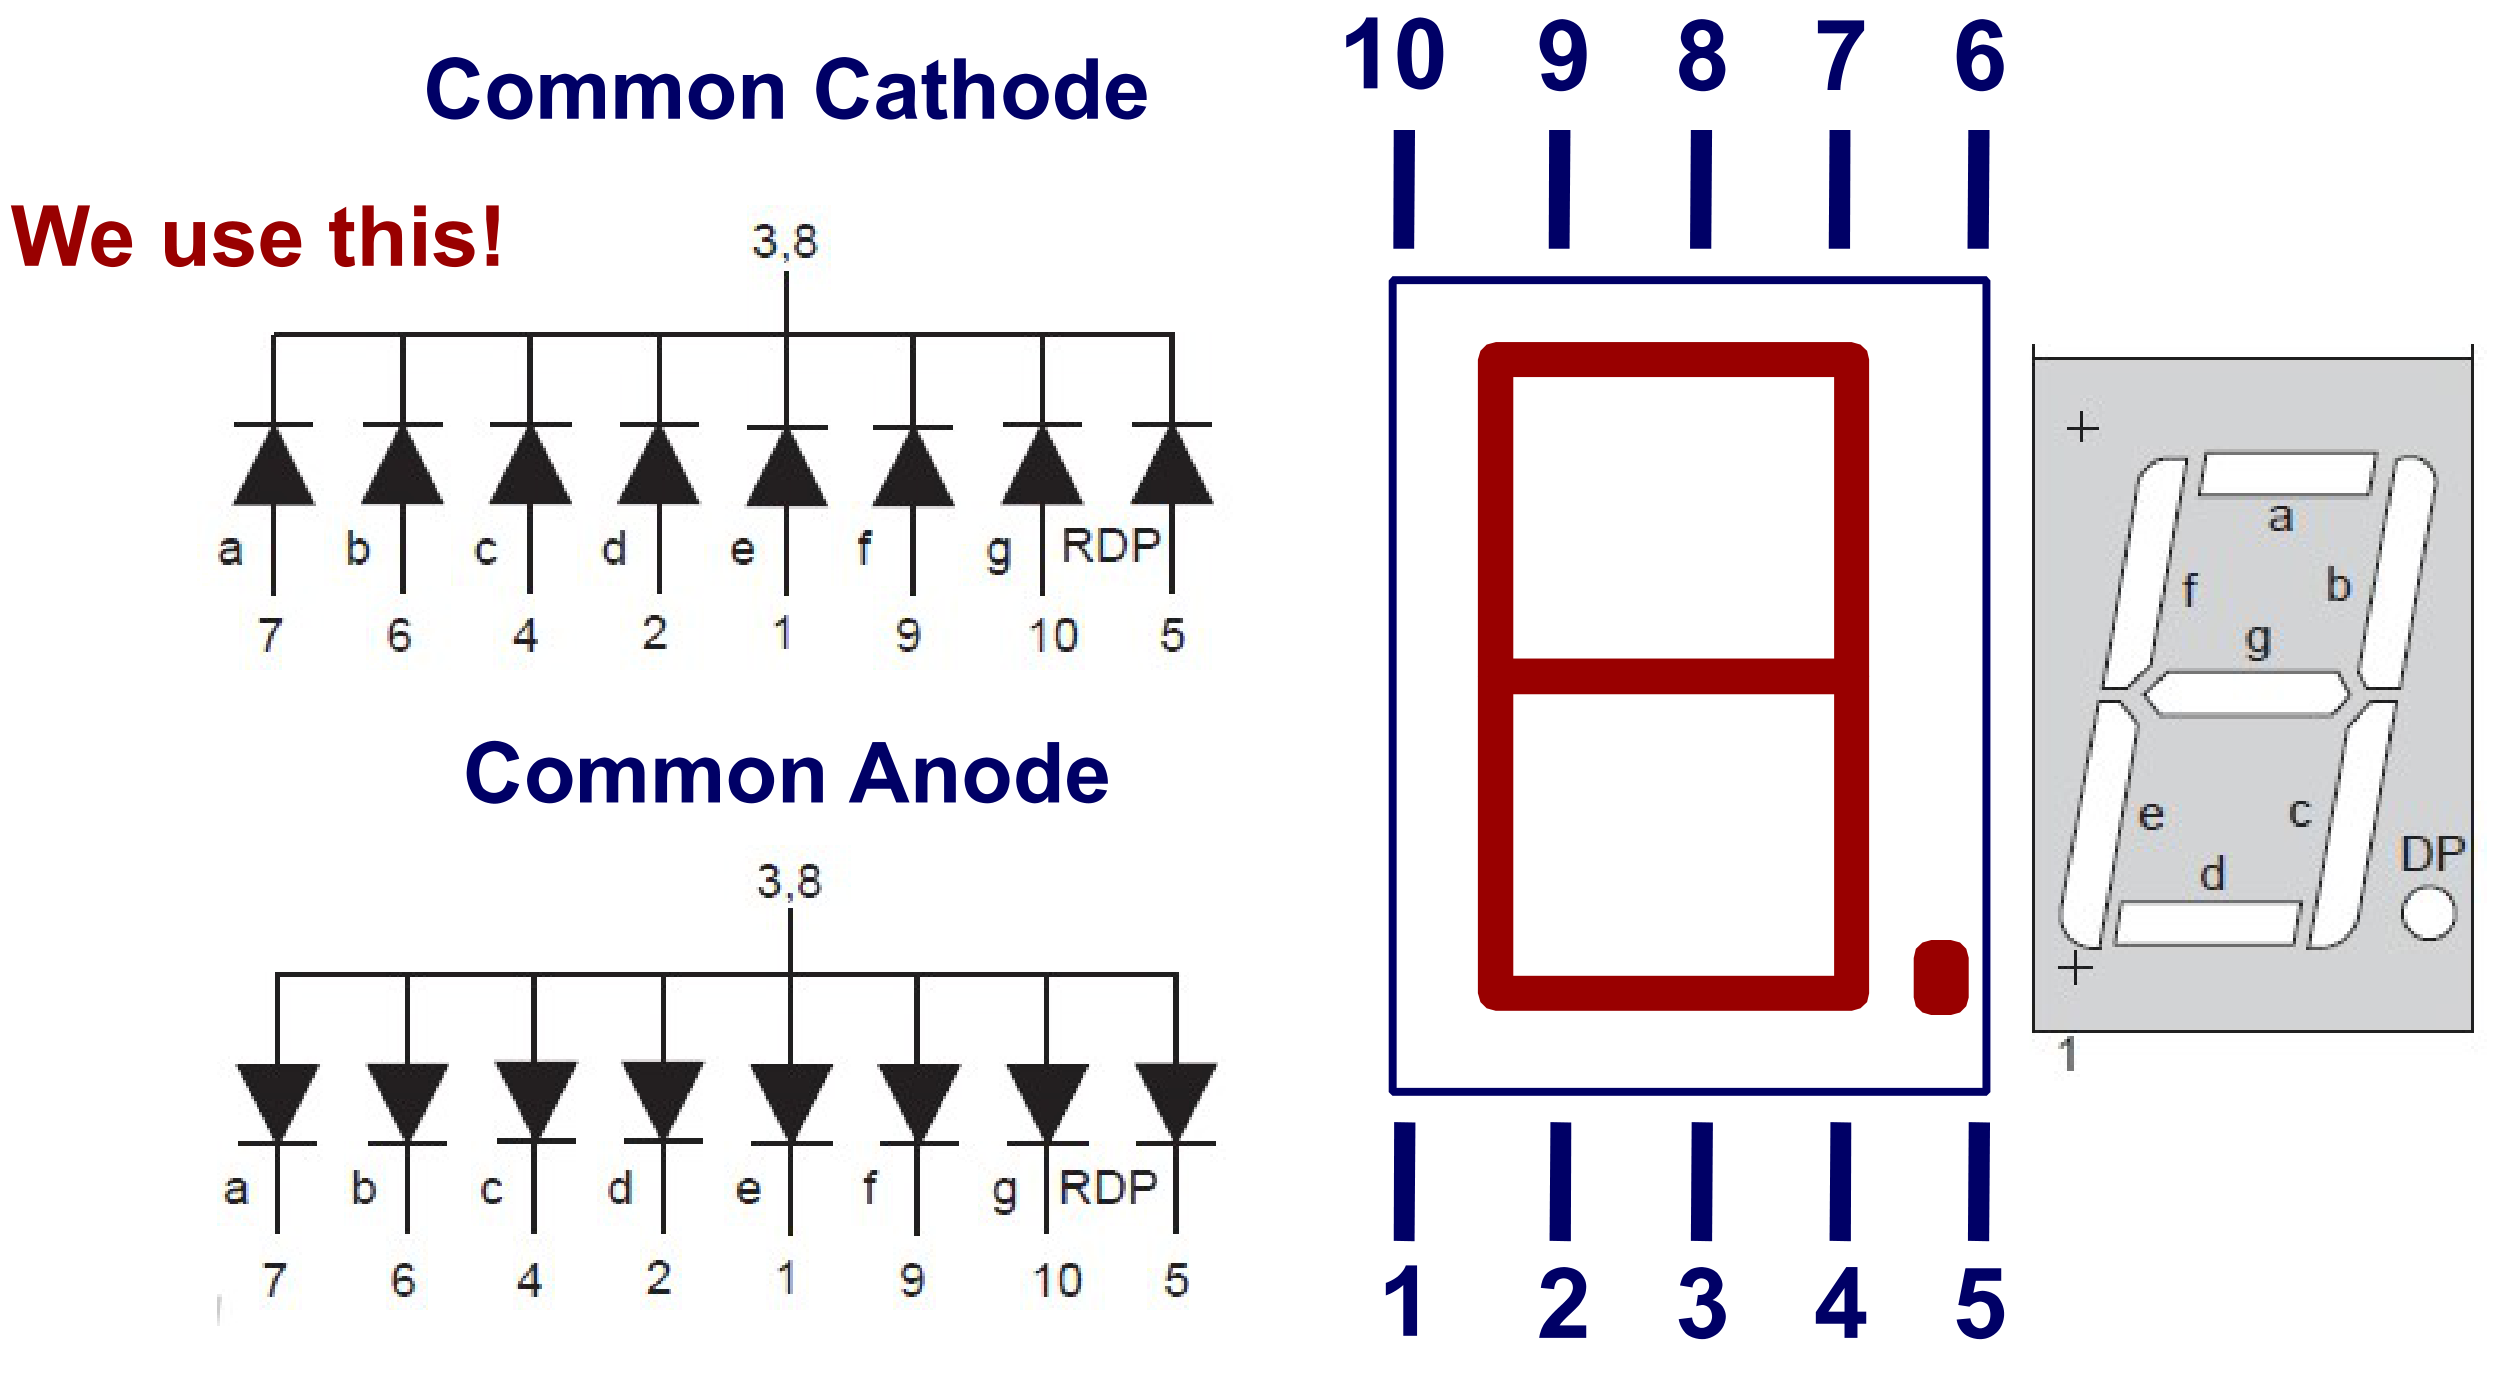
\includegraphics[width=\linewidth]{pic/7seg_types.png}
    \end{minipage}
    \hfill
    \begin{minipage}[c]{0.3\textwidth}
        \centering
        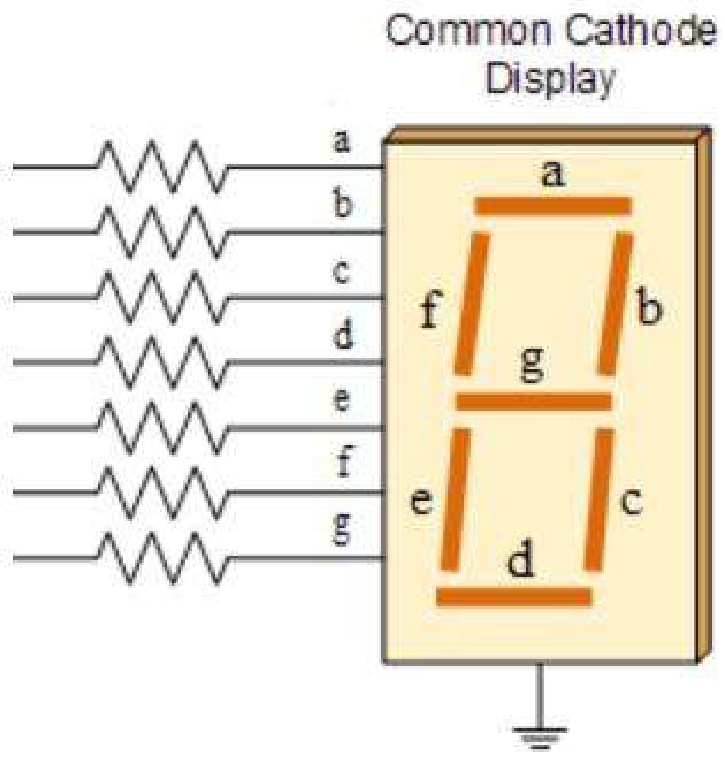
\includegraphics[width=\linewidth]{pic/7seg_cathode.png}
    \end{minipage}
    \captionof{figure}{Common-cathode / common-anode pin assignment (left) and connection with series resistors (right)}
    \label{fig:7seg}
\end{figure}
